\documentclass{beamer}

\usepackage{beamerthemesplit}
\usepackage{amsmath}
\usepackage{amsfonts}
\usepackage{amssymb}
\usepackage{qtree}
\usepackage{cancel}
\usepackage{tkz-graph}
%\usepackage[pdftex]{graphicx}

\makeatletter
\newcommand{\reallytiny}{\@setfontsize{\srcsize}{2pt}{2pt}}
\makeatother

\mode<presentation>
{
  \usetheme{metropolis}
  % or ...

  %\setbeamercovered{transparent}
  % or whatever (possibly just delete it)
}


\usepackage[english]{babel}
% or whatever

\usepackage[latin1]{inputenc}
% or whatever

\usepackage{times}
\usepackage[T1]{fontenc}

\title{Unified Rule Engine}
\subtitle{Inference Control Meta-Learning}

\author{Nil Geisweiller}

\institute[SingularityNET Foundation] % (optional, but mostly needed)
{
  SingularityNET Foundation
}

\date[SNETAthon Fall 018] % (optional, should be abbreviation of conference name)
{SNETAthon Fall 2018}


\AtBeginSection[]
{
  \begin{frame}<beamer>{Outline}
    \tableofcontents[currentsection,currentsection]
  \end{frame}
}

\AtBeginSubsection[]
{
  \begin{frame}<beamer>{Outline}
    \tableofcontents[currentsection,currentsubsection]
  \end{frame}
}

%\newcommand{\AND}{\textit{AND}}
%\newcommand{\OR}{\textit{OR}}
%\newcommand{\NOT}{\textit{NOT}}
\newcommand{\AND}{\land}
\newcommand{\OR}{\lor}
\newcommand{\NOT}{\lnot}


\begin{document}

\frame
{
  \maketitle
}

\begin{frame}[fragile]
  \frametitle{Unified Rule Engine: reminder}
  The URE \alert{evolves Inference Trees}
{\tiny \begin{semiverbatim}
\textcolor{blue}{A  A->B}
----------(MP)      
   \textcolor{red}{B}
\end{semiverbatim}}

{\tiny \begin{semiverbatim}
    \textcolor{blue}{A->B  B->C}
    ---------------(DED)
\textcolor{blue}{A}      A->C       
----------------(MP)   
     \textcolor{red}{C}
\end{semiverbatim}}

{\tiny \begin{semiverbatim}
\textcolor{blue}{ForAll X P(X)  U(P(X), A)        A->B  B->C}
--------------------------------------(INS)   ---------------(DED)
            A                       A->C       
            ------------------------------------------(MP)
                           \textcolor{red}{C}
\end{semiverbatim}}

\begin{itemize}
\item Leaves are \textcolor{blue}{premises}
\item Roots are \textcolor{red}{conclusions}
\end{itemize}
  
\end{frame}

\begin{frame}[fragile]
  \frametitle{URE: Unified Rule Engine}
  Inference Trees are constructed by composing \alert{Rules}
  \begin{itemize}
  \item<1-> \textcolor{red}{forward}: expand conclusion
    \begin{columns}
      \column{0.4in}
{\tiny \begin{semiverbatim}
\textcolor{blue}{A  A->B}
----------(MP)      
   \textcolor{red}{{\bf B}}
\end{semiverbatim}}
\column{0.1in}
$\Rightarrow$
\column{2in}
{\tiny \begin{semiverbatim}
\textcolor{blue}{A   A->B}
------------(MP)      
   {\bf B}        \textcolor{blue}{B->C}
   -------------------(MP)
          \textcolor{red}{C}
\end{semiverbatim}}
\end{columns}

\item<2-> \textcolor{blue}{backward}: expand premises
\begin{columns}
\column{0.4in}
{\tiny \begin{semiverbatim}
\textcolor{blue}{{\bf A}  A->B}
----------(MP)      
   \textcolor{red}{B}

\end{semiverbatim}}
\column{0.1in}
$\Rightarrow$
\column{2in}
{\tiny \begin{semiverbatim}
\textcolor{blue}{ForAll X P(X)  U(P(X), A)}
--------------------------------------(INS)
            {\bf A}                       \textcolor{blue}{A->B}
            ------------------------------------------(MP)
                           \textcolor{red}{B}

\end{semiverbatim}}
\end{columns}

\begin{columns}
  \column{0.4in}
{\tiny \begin{semiverbatim}
\textcolor{blue}{A  {\bf A->B}}
----------(MP)      
   \textcolor{red}{B}
\end{semiverbatim}}
\column{0.1in}
$\Rightarrow$
\column{2in}
{\tiny \begin{semiverbatim}
        \textcolor{blue}{A->C   C->B}
        -----------------(DED)
\textcolor{blue}{A}          {\bf A->B}
-----------------------(MP)
       \textcolor{red}{B}
\end{semiverbatim}}
\end{columns}

  \end{itemize}
\end{frame}

\begin{frame}[fragile]
  \frametitle{URE: Unified Rule Engine}
  Inference Trees are \alert{Atomese} Programs

  \begin{columns}
    \column{0.1in}

    \begin{onlyenv}<1-2>
    
{\tiny \begin{semiverbatim}
\textcolor{blue}{A  A->B}
----------(MP)      
   \textcolor{red}{B}
\end{semiverbatim}}

\end{onlyenv}

\begin{onlyenv}<3>

{\tiny \begin{semiverbatim}
     \textcolor{blue}{A->C   C->B}
     -----------------(DED)
\textcolor{blue}{A}       \textcolor{violet}{A->B}
------------------(MP)
     \textcolor{red}{B}
\end{semiverbatim}}

\end{onlyenv}

\column{2in}

\begin{onlyenv}<1>

{\TINY
\begin{verbatim}
(BindLink
  (VariableList                                             \
    (TypedVariableLink                                      |
      (VariableNode "$A")                                   |
      (TypeChoice                                           |
        (TypeNode "LambdaLink")                             |
        (TypeNode "PredicateNode")                          |
      )                                                     |
    )                                                       | Variables
    (TypedVariableLink                                      |
      (VariableNode "$B")                                   |
      (TypeChoice                                           |
        (TypeNode "LambdaLink")                             |
        (TypeNode "PredicateNode")                          |
      )                                                     |
    )                                                       |
  )                                                         /
  (AndLink                                                  \
    (ImplicationLink                                        |
      (VariableNode "$A")                                   | Pattern
      (VariableNode "$B")                                   |
    )                                                       /
    (EvaluationLink                                         \
      (GroundedPredicateNode "scm: true-enough")            |
      (ImplicationLink                                      |
        (VariableNode "$A")                                 |
        (VariableNode "$B")                                 |
      )                                                     |
    )                                                       | Preconditions
    (EvaluationLink                                         |
      (GroundedPredicateNode "scm: true-enough")            |
      (VariableNode "$A")                                   |
    )                                                       |
  )                                                         /
  (ExecutionOutputLink                                      \
    (GroundedSchemaNode "scm: modus-ponens-formula")        |
    (ListLink                                               |
      (VariableNode "$B")                                   |
      (VariableNode "$A")                                   |
      (ImplicationLink                                      | Production
        (VariableNode "$A")                                 |
        (VariableNode "$B")                                 |
      )                                                     |
    )                                                       |
  )                                                         /
)
\end{verbatim}
}

\end{onlyenv}

\begin{onlyenv}<2>

  {\tiny
\begin{semiverbatim}




  


  
  (ExecutionOutputLink                                    
    (GroundedSchemaNode "scm: modus-ponens-formula")
    (ListLink                                             
      \textcolor{red}{(VariableNode "$B")}
      \textcolor{blue}{(VariableNode "$A")
      (ImplicationLink
        (VariableNode "$A")
        (VariableNode "$B")
      )}
    )
  )







\end{semiverbatim}
}

\end{onlyenv}

\begin{onlyenv}<3>

  {\tiny
\begin{semiverbatim}
  (ExecutionOutputLink                                    
    (GroundedSchemaNode "scm: modus-ponens-formula")
    (ListLink                                             
      \textcolor{red}{(VariableNode "$B")}
      \textcolor{blue}{(VariableNode "$A")}
      (ExecutionOutputLink
        (GroundedSchemaNode "scm: deduction-formula")
        (ListLink
          \textcolor{violet}{(ImplicationLink
            (VariableNode "$A")
            (VariableNode "$B")
          )}
          \textcolor{blue}{(ImplicationLink
            (VariableNode "$A")
            (VariableNode "$C")
          )
          (ImplicationLink
            (VariableNode "$C")
            (VariableNode "$B")
          )}
        )
      )
    )
  )
\end{semiverbatim}
}

\end{onlyenv}

\end{columns}

\end{frame}

\begin{frame}
  \frametitle{URE: Unified Rule Engine}

  Algorithm
  \begin{enumerate}
  \item \alert{Select an inference tree} to expand
  \item \alert{Select a node} from that tree to expand
  \item \alert{Select a rule} to expand with
  \item Expand the inference tree and place it back to the pool of
    inference trees. Repeat till termination.
  \end{enumerate}

  \begin{center}
    \textcolor{red}{Combinatorial Explosion}
  \end{center}
  
\end{frame}
  
\begin{frame}[fragile]
  \frametitle{Inference Control}

  \begin{center}
    Delegate the hard decisions to a \alert{cognitive process}
  \end{center}

  Cognitive Schematics:
  $$\textcolor{blue}{\text{Context}}\ \&\ \textcolor{red}{\text{Action}}\ \Rightarrow\ \textcolor{green}{\text{Goal}}$$

  {\small
Atomese:
\begin{semiverbatim}
Implication <TV>
  And
    \textcolor{blue}{<Context>}
    \textcolor{red}{<Action>}
  \textcolor{green}{<Goal>}
\end{semiverbatim}
}

\end{frame}

\begin{frame}[fragile]
  \frametitle{Inference Control}

  \begin{columns}
    \column{0.4in}
{\tiny \begin{semiverbatim}






\textcolor{blue}{{\bf A}  A->B}
----------(MP)      
   \textcolor{red}{B}




\end{semiverbatim}}
\column{2in}
Which rule to choose?
\begin{enumerate}
\item Modus Ponens
\item Universal Instantiation
\end{enumerate}
\end{columns}

Look for:
{\small
\begin{semiverbatim}
Implication <TV>
  And
    \textcolor{blue}{<inference-tree-pattern>
    <node-pattern>}
    \textcolor{red}{<rule-pattern>}
  \textcolor{green}{<produce-good-inference>}
\end{semiverbatim}
}

\end{frame}

\begin{frame}[fragile]
  \frametitle{Inference Control}

  Examples of actual URE Cognitive Schematics
  
  \begin{columns}
    \column{2in}

{\TINY
\begin{semiverbatim}
(ImplicationScopeLink (stv 0.45945946 0.04625)
   (VariableList
      (VariableNode "$T")
      (TypedVariableLink
         (VariableNode "$A")
         (TypeNode "DontExecLink")
      )
      (VariableNode "$L")
      (TypedVariableLink
         (VariableNode "$B")
         (TypeNode "DontExecLink")
      )
   )
   (AndLink
      \textcolor{blue}{(EvaluationLink
         (PredicateNode "URE:BC:preproof-of")
         (ListLink
            (VariableNode "$A")
            (VariableNode "$T")
         )
      )
      (ExecutionLink
         (SchemaNode "URE:BC:expand-and-BIT")
         (ListLink
            (VariableNode "$A")
            (VariableNode "$L")
            \textcolor{red}{(DontExecLink
               (DefinedSchemaNode "deduction-inheritance-rule")
            )}
         )
         (VariableNode "$B")
      )}
   )
   \textcolor{green}{(EvaluationLink
      (PredicateNode "URE:BC:preproof-of")
      (ListLink
         (VariableNode "$B")
         (VariableNode "$T")
      )
   )}
)
\end{semiverbatim}
}

    \column{2in}

{\TINY
\begin{semiverbatim}
(ImplicationScopeLink (stv 1 0.00625)
   (VariableList
      (VariableNode "$T")
      (TypedVariableLink
         (VariableNode "$A")
         (TypeNode "DontExecLink")
      )
      (VariableNode "$X")
      (TypedVariableLink
         (VariableNode "$B")
         (TypeNode "DontExecLink")
      )
   )
   (AndLink
      \textcolor{blue}{(EvaluationLink
         (PredicateNode "URE:BC:preproof-of")
         (ListLink
            (VariableNode "$A")
            (VariableNode "$T")
         )
      )
      (ExecutionLink
         (SchemaNode "URE:BC:expand-and-BIT")
         (ListLink
            (VariableNode "$A")
            (InheritanceLink
               (ConceptNode "a")
               (VariableNode "$X")
            )
            \textcolor{red}{(DontExecLink
               (DefinedSchemaNode "conditional-full-instantiation-implication-scope-meta-rule")
            )}
         )
         (VariableNode "$B")
      )}
   )
   \textcolor{green}{(EvaluationLink
      (PredicateNode "URE:BC:preproof-of")
      (ListLink
         (VariableNode "$B")
         (VariableNode "$T")
      )
   )}
)
\end{semiverbatim}
}

\end{columns}

\end{frame}

\begin{frame}
  \frametitle{Inference Control Algorithm}

  Given:
  \begin{itemize}
  \item \textcolor{red}{inference rules}: $R_1$, ..., $R_n$
  \item \textcolor{red}{control rules}:
    \begin{itemize}
    \item $R_1$ $\rightarrow$ $\{$ $C_{1,1}$, ..., $C_{1,m_1}$ $\}$
    \item ...
    \item $R_n$ $\rightarrow$ $\{$ $C_{n,1}$, ..., $C_{n,m_n}$ $\}$
    \end{itemize}
  \end{itemize}

  \begin{center}
    \alert{Combine $C_{i,j}$ to select best $R_i$}\\
    ?
  \end{center}

\end{frame}

\begin{frame}
  \frametitle{Inference Control Algorithm}
  Selecting inference rule $R_i$:
  \begin{enumerate}
  \item \textcolor{red}{Mixture model}:
    $M_i = C_{i, 1} \oplus \dots \oplus C_{i, m_i}$\\
    (Bayesian Model Averaging, Solomonoff Operator Induction).
  \item \textcolor{red}{Thomspon Sampling}: $R_i = TS(M_1, \dots, M_n)$
  \end{enumerate}
  \begin{center}
    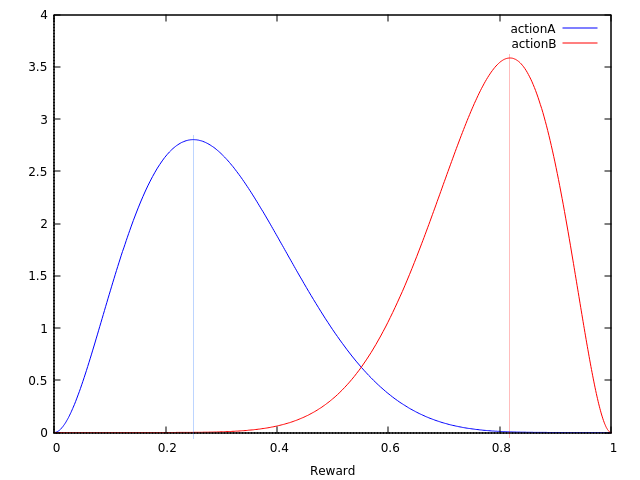
\includegraphics[scale=0.4]{ActionA_ActionB_lines_alpha.png}
  \end{center}

\end{frame}

\begin{frame}
  \frametitle{Inference Control Meta-Learning}

  How to get Control Rules?

  Answer: \textcolor{red}{Learning}

  \begin{center}
    \alert{Record all decisions}\\
    the URE takes and \alert{learn} from it
  \end{center}

  Currently: \textcolor{red}{Pattern Mining}

\end{frame}

\begin{frame}[fragile]
  \frametitle{Inference Control Learning: URE Trace}

\begin{columns}
\column{.6in}
{\tiny \begin{semiverbatim}
\textcolor{blue}{A  {\bf A->B}}
----------(MP)      
   \textcolor{red}{B}
\end{semiverbatim}}
\column{0.1in}
{\Tiny Expand}
$\rightarrow$
\column{2in}
{\tiny \begin{semiverbatim}
        \textcolor{blue}{A->C   C->B}
        -----------------(DED)
\textcolor{blue}{A}          {\bf A->B}
-----------------------(MP)
       \textcolor{red}{B}
\end{semiverbatim}}
\end{columns}

{\tiny Atomese:}

\begin{columns}

\column{1in}
  
{\reallytiny
\begin{semiverbatim}
(ExecutionLink (stv 1 1)
   (SchemaNode "URE:BC:expand-and-BIT")
   (ListLink
      (DontExecLink
         (BindLink
            (VariableNode "$A-591b9032")
            (AndLink
               (VariableNode "$A-591b9032")
               (InheritanceLink
                  (VariableNode "$A-591b9032")
                  (InheritanceLink (stv 1 1)
                     (ConceptNode "v" (stv 0.84615385 1))
                     (ConceptNode "w")
                  )
               )
               (EvaluationLink
                  (GroundedPredicateNode "scm: gt-zero-confidence")
                  (VariableNode "$A-591b9032")
               )
               (EvaluationLink
                  (GroundedPredicateNode "scm: gt-zero-confidence")
                  (InheritanceLink
                     (VariableNode "$A-591b9032")
                     (InheritanceLink (stv 1 1)
                        (ConceptNode "v" (stv 0.84615385 1))
                        (ConceptNode "w")
                     )
                  )
               )
            )
            (ExecutionOutputLink
               (GroundedSchemaNode "scm: modus-ponens-formula")
               (ListLink
                  (InheritanceLink (stv 1 1)
                     (ConceptNode "v" (stv 0.84615385 1))
                     (ConceptNode "w")
                  )
                  (InheritanceLink
                     (VariableNode "$A-591b9032")
                     (InheritanceLink (stv 1 1)
                        (ConceptNode "v" (stv 0.84615385 1))
                        (ConceptNode "w")
                     )
                  )
                  (VariableNode "$A-591b9032")
               )
            )
         )
      )
      (VariableNode "$A-1860e3b6")
      (DontExecLink
         (DefinedSchemaNode "deduction-inheritance-rule")
      )
   )
\end{semiverbatim}}

\column{1in}

{\reallytiny
\begin{semiverbatim}
   (DontExecLink
      (BindLink
         (VariableList
            (TypedVariableLink
               (VariableNode "$A-2fbf17d5")
               (TypeChoice
                  (TypeNode "ConceptNode")
                  (TypeNode "AndLink")
                  (TypeNode "OrLink")
                  (TypeNode "NotLink")
               )
            )
            (TypedVariableLink
               (VariableNode "$C-2bdc1299")
               (TypeChoice
                  (TypeNode "ConceptNode")
                  (TypeNode "AndLink")
                  (TypeNode "OrLink")
                  (TypeNode "NotLink")
               )
            )
            (TypedVariableLink
               (VariableNode "$B-4a714efb")
               (TypeChoice
                  (TypeNode "ConceptNode")
                  (TypeNode "AndLink")
                  (TypeNode "OrLink")
                  (TypeNode "NotLink")
               )
            )
         )
         (AndLink
            (EvaluationLink
               (GroundedPredicateNode "scm: gt-zero-confidence")
               (InheritanceLink
                  (InheritanceLink
                     (VariableNode "$A-2fbf17d5")
                     (VariableNode "$C-2bdc1299")
                  )
                  (InheritanceLink (stv 1 1)
                     (ConceptNode "v" (stv 0.84615385 1))
                     (ConceptNode "w")
                  )
               )
            )
            (InheritanceLink
               (VariableNode "$B-4a714efb")
               (VariableNode "$C-2bdc1299")
            )
            (InheritanceLink
               (InheritanceLink
                  (VariableNode "$A-2fbf17d5")
                  (VariableNode "$C-2bdc1299")
               )
               (InheritanceLink (stv 1 1)
                  (ConceptNode "v" (stv 0.84615385 1))
                  (ConceptNode "w")
               )
            )
            (NotLink
               (IdenticalLink
                  (VariableNode "$C-2bdc1299")
                  (VariableNode "$A-2fbf17d5")
               )
            )
            (InheritanceLink
               (VariableNode "$A-2fbf17d5")
               (VariableNode "$B-4a714efb")
            )
         )
\end{semiverbatim}}

\column{1in}

{\reallytiny
\begin{semiverbatim}
         (ExecutionOutputLink
            (GroundedSchemaNode "scm: modus-ponens-formula")
            (ListLink
               (InheritanceLink (stv 1 1)
                  (ConceptNode "v" (stv 0.84615385 1))
                  (ConceptNode "w")
               )
               (InheritanceLink
                  (InheritanceLink
                     (VariableNode "$A-2fbf17d5")
                     (VariableNode "$C-2bdc1299")
                  )
                  (InheritanceLink (stv 1 1)
                     (ConceptNode "v" (stv 0.84615385 1))
                     (ConceptNode "w")
                  )
               )
               (ExecutionOutputLink
                  (GroundedSchemaNode "scm: deduction-formula")
                  (ListLink
                     (InheritanceLink
                        (VariableNode "$A-2fbf17d5")
                        (VariableNode "$C-2bdc1299")
                     )
                     (InheritanceLink
                        (VariableNode "$A-2fbf17d5")
                        (VariableNode "$B-4a714efb")
                     )
                     (InheritanceLink
                        (VariableNode "$B-4a714efb")
                        (VariableNode "$C-2bdc1299")
                     )
                  )
               )
            )
         )
      )
   )
)
\end{semiverbatim}
}

\end{columns}

\end{frame}

\begin{frame}[fragile]
  \frametitle{Inference Control Learning: URE Trace}

\begin{columns}
\column{1in}
{\tiny \begin{semiverbatim}
       \textcolor{blue}{A->C   C->B}
       -----------------(DED)
\textcolor{blue}{A}          A->B
-----------------------(MP)
       \textcolor{red}{B}
\end{semiverbatim}}
\column{0.1in}
{\Tiny Quality}
$\rightarrow$
\column{2in}
{\tiny (stv $0.0001$, $0.00075$)}

\end{columns}

{\tiny Atomese:}

\begin{columns}

\column{1in}
  
{\reallytiny
\begin{semiverbatim}
(EvaluationLink (stv 0.0001 0.00075)
   (PredicateNode "URE:BC:preproof-of")
   (ListLink
      (DontExecLink
         (BindLink
            (VariableList
               (TypedVariableLink
                  (VariableNode "$A-2fbf17d5")
                  (TypeChoice
                     (TypeNode "ConceptNode")
                     (TypeNode "AndLink")
                     (TypeNode "OrLink")
                     (TypeNode "NotLink")
                  )
               )
               (TypedVariableLink
                  (VariableNode "$C-2bdc1299")
                  (TypeChoice
                     (TypeNode "ConceptNode")
                     (TypeNode "AndLink")
                     (TypeNode "OrLink")
                     (TypeNode "NotLink")
                  )
               )
               (TypedVariableLink
                  (VariableNode "$B-4a714efb")
                  (TypeChoice
                     (TypeNode "ConceptNode")
                     (TypeNode "AndLink")
                     (TypeNode "OrLink")
                     (TypeNode "NotLink")
                  )
               )
            )
            (AndLink
               (EvaluationLink
                  (GroundedPredicateNode "scm: gt-zero-confidence")
                  (InheritanceLink
                     (InheritanceLink
                        (VariableNode "$A-2fbf17d5")
                        (VariableNode "$C-2bdc1299")
                     )
                     (InheritanceLink (stv 1 1)
                        (ConceptNode "v" (stv 0.84615385 1))
                        (ConceptNode "w")
                     )
                  )
               )
               (InheritanceLink
                  (VariableNode "$B-4a714efb")
                  (VariableNode "$C-2bdc1299")
               )
               (InheritanceLink
                  (InheritanceLink
                     (VariableNode "$A-2fbf17d5")
                     (VariableNode "$C-2bdc1299")
                  )
                  (InheritanceLink (stv 1 1)
                     (ConceptNode "v" (stv 0.84615385 1))
                     (ConceptNode "w")
                  )
               )
               (NotLink
                  (IdenticalLink
                     (VariableNode "$C-2bdc1299")
                     (VariableNode "$A-2fbf17d5")
                  )
               )
               (InheritanceLink
                  (VariableNode "$A-2fbf17d5")
                  (VariableNode "$B-4a714efb")
               )
            )
\end{semiverbatim}}

\column{1in}
               
{\reallytiny
\begin{semiverbatim}
            (ExecutionOutputLink
               (GroundedSchemaNode "scm: modus-ponens-formula")
               (ListLink
                  (InheritanceLink (stv 1 1)
                     (ConceptNode "v" (stv 0.84615385 1))
                     (ConceptNode "w")
                  )
                  (InheritanceLink
                     (InheritanceLink
                        (VariableNode "$A-2fbf17d5")
                        (VariableNode "$C-2bdc1299")
                     )
                     (InheritanceLink (stv 1 1)
                        (ConceptNode "v" (stv 0.84615385 1))
                        (ConceptNode "w")
                     )
                  )
                  (ExecutionOutputLink
                     (GroundedSchemaNode "scm: deduction-formula")
                     (ListLink
                        (InheritanceLink
                           (VariableNode "$A-2fbf17d5")
                           (VariableNode "$C-2bdc1299")
                        )
                        (InheritanceLink
                           (VariableNode "$A-2fbf17d5")
                           (VariableNode "$B-4a714efb")
                        )
                        (InheritanceLink
                           (VariableNode "$B-4a714efb")
                           (VariableNode "$C-2bdc1299")
                        )
                     )
                  )
               )
            )
         )
      )
      (InheritanceLink (stv 1 1)
         (ConceptNode "v" (stv 0.84615385 1))
         (ConceptNode "w")
      )
   )
)
\end{semiverbatim}}

\end{columns}

\end{frame}

\begin{frame}[fragile]
  \frametitle{Inference Control Learning: URE \visible<3>{+ Pattern Miner}}

  {\small Call the URE with a Control Rule Template as target \visible<3>{+
    Pattern Miner}}

\begin{columns}

\column{2in}
  
{\Tiny \begin{semiverbatim}


(cog-bc icr-rb (QuoteLink
                  (ImplicationScopeLink
                     (UnquoteLink
                        (VariableNode "$impl-vardecl")
                     )
                     (AndLink
                        (EvaluationLink
                           (PredicateNode "URE:BC:preproof-of")
                           (UnquoteLink
                              (VariableNode "$preproof-A-args")
                           )
                        )
                        (ExecutionLink
                           (SchemaNode "URE:BC:expand-and-BIT")
                           (UnquoteLink
                              (VariableNode "$expand-inputs")
                           )
                           (UnquoteLink
                              (VariableNode "$expand-output")
                           )
                        )
                     )
                     (EvaluationLink
                        (PredicateNode "URE:BC:preproof-of")
                        (UnquoteLink
                           (VariableNode "$preproof-B-args")
                        )
                     )
                  )
               )
            )



\end{semiverbatim}}

\column{2in}

\begin{onlyenv}<2>

{\TINY
\begin{semiverbatim}
(ImplicationScopeLink (stv 0.45945946 0.04625)
   (VariableList
      (VariableNode "$T")
      (TypedVariableLink
         (VariableNode "$A")
         (TypeNode "DontExecLink")
      )
      (VariableNode "$L")
      (TypedVariableLink
         (VariableNode "$B")
         (TypeNode "DontExecLink")
      )
   )
   (AndLink
      \textcolor{blue}{(EvaluationLink
         (PredicateNode "URE:BC:preproof-of")
         (ListLink
            (VariableNode "$A")
            (VariableNode "$T")
         )
      )
      (ExecutionLink
         (SchemaNode "URE:BC:expand-and-BIT")
         (ListLink
            (VariableNode "$A")
            (VariableNode "$L")
            \textcolor{red}{(DontExecLink
               (DefinedSchemaNode "deduction-inheritance-rule")
            )}
         )
         (VariableNode "$B")
      )}
   )
   \textcolor{green}{(EvaluationLink
      (PredicateNode "URE:BC:preproof-of")
      (ListLink
         (VariableNode "$B")
         (VariableNode "$T")
      )
   )}
)
\end{semiverbatim}
}

\end{onlyenv}

\begin{onlyenv}<3>

{\TINY
\begin{semiverbatim}
(ImplicationScopeLink (stv 1 0.00625)
   (VariableList
      (VariableNode "$T")
      (TypedVariableLink
         (VariableNode "$A")
         (TypeNode "DontExecLink")
      )
      (VariableNode "$X")
      (TypedVariableLink
         (VariableNode "$B")
         (TypeNode "DontExecLink")
      )
   )
   (AndLink
      \textcolor{blue}{(EvaluationLink
         (PredicateNode "URE:BC:preproof-of")
         (ListLink
            (VariableNode "$A")
            (VariableNode "$T")
         )
      )
      (ExecutionLink
         (SchemaNode "URE:BC:expand-and-BIT")
         (ListLink
            (VariableNode "$A")
            (InheritanceLink
               (ConceptNode "a")
               (VariableNode "$X")
            )
            \textcolor{red}{(DontExecLink
               (DefinedSchemaNode "conditional-full-instantiation-implication-scope-meta-rule")
            )}
         )
         (VariableNode "$B")
      )}
   )
   \textcolor{green}{(EvaluationLink
      (PredicateNode "URE:BC:preproof-of")
      (ListLink
         (VariableNode "$B")
         (VariableNode "$T")
      )
   )}
)
\end{semiverbatim}
}

\end{onlyenv}

\end{columns}

\end{frame}

\begin{frame}
  \frametitle{Issues, forthcoming work}

  \begin{itemize}
  \item Issues:
    \begin{itemize}
    \item Pattern Miner (WIP), \alert{looking for challenges!}
    \item Too many control rules?
    \end{itemize}
  \item Forthcoming:
    \begin{itemize}
    \item Experimentations, \alert{looking for challenges!}
    \item Other learning methods, MOSES, etc
    \item Integrate ECAN
    \end{itemize}
  \end{itemize}

  \pause
  
  \begin{center}
    \textcolor{green}{Demo time...}
  \end{center}
\end{frame}

\end{document}
